\documentclass[12pt]{article}
\usepackage[top=1in,left=1in, right = 1in, footskip=1in]{geometry}

\usepackage{graphicx}
\usepackage{xspace}
%\usepackage{adjustbox}

\newcommand{\comment}{\showcomment}
%% \newcommand{\comment}{\nocomment}

\newcommand{\showcomment}[3]{\textcolor{#1}{\textbf{[#2: }\textsl{#3}\textbf{]}}}
\newcommand{\nocomment}[3]{}

\newcommand{\jd}[1]{\comment{cyan}{JD}{#1}}
\newcommand{\swp}[1]{\comment{magenta}{SWP}{#1}}
\newcommand{\bmb}[1]{\comment{blue}{BMB}{#1}}
\newcommand{\djde}[1]{\comment{red}{DJDE}{#1}}
\newcommand{\old}{\sffamily}
\newcommand{\told}{\textsf}

\newcommand{\eref}[1]{Eq.~\ref{eq:#1}}
\newcommand{\fref}[1]{Fig.~\ref{fig:#1}}
\newcommand{\Fref}[1]{Fig.~\ref{fig:#1}}
\newcommand{\sref}[1]{Sec.~\ref{#1}}
\newcommand{\frange}[2]{Fig.~\ref{fig:#1}--\ref{fig:#2}}
\newcommand{\tref}[1]{Table~\ref{tab:#1}}
\newcommand{\tlab}[1]{\label{tab:#1}}
\newcommand{\pday}{\ensuremath{/\textrm{day}}}

\usepackage{amsthm}
\usepackage{amsmath}
\usepackage{amssymb}
\usepackage{amsfonts}

\usepackage{lineno}
\linenumbers

\usepackage[pdfencoding=auto, psdextra]{hyperref}

\usepackage{natbib}
\bibliographystyle{chicago}
\date{\today}

\usepackage{xspace}
\newcommand*{\ie}{i.e.\@\xspace}

\usepackage{color}

\newcommand{\Rx}[1]{\ensuremath{{\mathcal R}_{#1}}\xspace} 
\newcommand{\Ro}{\Rx{0}}
\newcommand{\Rc}{\Rx{\mathrm{c}}}
\newcommand{\Ri}{\Rx{\mathrm{i}}}
\newcommand{\RR}{\ensuremath{{\mathcal R}}\xspace}
\newcommand{\Rhat}{\ensuremath{{\hat\RR}}}
\newcommand{\Rprop}{\Rx{\mathrm{prop}}}
\newcommand{\Rcori}{\Rx{\mathrm{cori}}}
\newcommand{\tsub}[2]{#1_{{\textrm{\tiny #2}}}}
\newcommand{\dd}[1]{\ensuremath{\, \mathrm{d}#1}}
\newcommand{\dtau}{\dd{\tau}}
\newcommand{\dx}{\dd{x}}
\newcommand{\dsigma}{\dd{\sigma}}

\newcommand{\tstart}{\ensuremath{\tsub{t}{start}}\xspace}
\newcommand{\tend}{\ensuremath{\tsub{t}{end}}\xspace}

\newcommand{\betaeff}{\ensuremath{\tsub{\beta}{eff}}\xspace}
\newcommand{\Keff}{\ensuremath{\tsub{K}{eff}}\xspace}
\newcommand{\Kpost}{\ensuremath{\tsub{K}{post}}\xspace}

\newcommand{\pt}{p} %% primary time
\newcommand{\st}{s} %% secondary time

\newcommand{\psize}{{\mathcal P}} %% primary cohort size
\newcommand{\ssize}{{\mathcal S}} %% secondary cohort size

\newcommand{\gtime}{\sigma} %% generation interval
\newcommand{\gdist}{g} %% generation-interval distribution

\newcommand{\geff}{g_{\textrm{eff}}} %% generation-interval distribution

\newcommand{\total}{{\mathcal T}} %% total number of serial intervals

\newcommand{\PP}{\ensuremath{\mathcal P}}
\newcommand{\II}{\ensuremath{\mathcal I}}
\newcommand{\HH}{\ensuremath{\mathcal H}}

\begin{document}

\begin{flushleft}{
	\Large
	\textbf\newline{
		Quantifying the effects of strength- and speed-like interventions on epidemic dynamics
	}
}
\newline
\\
Sang Woo Park\textsuperscript{1,*}, Kaiyuan Sun, Benjamin M. Bolker, Bryan T. Grenfell, Jonathan Dushoff, \swp{and others if needed}
\\
\bigskip
\textbf{1} Department of Ecology and Evolutionary Biology, Princeton University, Princeton, NJ, USA
\\
\bigskip

*Corresponding author: swp2@princeton.edu
\end{flushleft}

\section{Introduction}

\jd{The definitions are well done -- but I would like to play with them if I get a chance.}
The reproduction number \RR---typically defined as the average number of new infections caused by an infected individual---is a key characteristic of an emerging epidemic.
Its value in a fully susceptible population---the \emph{basic} reproduction number, \Ro---provides information about whether a pathogen can invade, the level of intervention required to prevent invasion, and the final size of an epidemic \citep{diekmann1990definition,anderson1991infectious}.
When an epidemic is ongoing, transmission dynamics are affected by changes in population-level immunity, non-pharmaceutical interventions, and contact patterns---these changes in transmission dynamics can be described by $\RR(t)$, often referred to as the \emph{effective} or \emph{time-dependent} reproduction number \citep{wallinga2004different, fraser2007estimating, cori2013new}.
Interpretation and estimation of $\RR(t)$ have been a key area of research during the ongoing COVID-19 pandemic due to its policy implications \citep{pan2020association,flaxman2020estimating,gostic2020practical}.

One of the main challenges in interpreting $\RR(t)$ can be attributed, in part, to its standard, heuristic definition: the average number of new infections caused by an infected individual.
While this definition is biologically intuitive, it is mathematically imprecise as time-dependent reproduction numbers can be defined in multiple ways, depending on the cohort (e.g., a group of individuals who developed symptoms or were infected at the same time) and the types of transmission scenarios (i.e., realized or counterfactual transmission processes).
Here, we primarily focus on two main measures of transmission that look at a cohort of infectees or infectors that were infected at the same time: the instantaneous reproduction number $\Ri(t)$ and the case reproduction number $\Rc(t)$.

First, the instantaneous reproduction number $\Ri(t)$---popularized by \cite{cori2013new}---was initially defined as the average number of new infections that an individual infected at time $t$ (i.e., an individual from a cohort of infectees) will generate over the course of their infection if conditions at time $t$ remain unchanged \citep{fraser2007estimating}. 
We further note that $\Ri(t)$ does not actually depend on when the person gets infected, only on when the conditions are held constant at---that is, if we freeze conditions at time $t$, anyone who become infected after time $t$ will cause same number of infections on average.
Therefore, the instantaneous reproduction number $\Ri(t)$ characterizes transmission conditions at time $t$ and provides a real-time estimate of whether the disease will continue to spread if conditions were to stay the same \citep{gostic2020practical}.
However, since transmission dynamics change throughout an epidemic, $\Ri(t)$ represents a counterfactual scenario and must be interpreted with care.

On the other hand, the case reproduction number $\Rc(t)$---popularized by \cite{wallinga2004different}---corresponds to the average number of new infections that an individual infected at time $t$ generated over the course of their infection.
$\Rc(t)$ is a realized measure, which depends on conditions after time $t$ and can only be estimated retrospectively.
Although the heuristic definition of $\RR(t)$ (``the average number of new infections caused by an infected individual'') closely resembles that of $\Rc(t)$, the mathematical definitions of $\RR(t)$ derived from standard compartmental models (e.g., basic reproduction multiplied by the proportion susceptible) actually correspond to that of $\Ri(t)$ \citep{gostic2020practical}.
Due to the imprecision of the heuristic definition of $\RR(t)$, the counterfactual quality of $\Ri(t)$ (and therefore, $\RR(t)$) is often neglected in its interpretation.
% \swp{return to this s. later}

Analogous to the reproduction number $\RR$, exponential growth rate $r$ describes the speed at which infection spreads at the population-level.
When conditions remain the same, both $\RR$ and $r$ provide equivalent threshold measures for control and are linked by the generation-interval distribution $g(\tau)$, where generation intervals describe time between infections of an infector and an infectee \citep{svensson2007note}.
Throuhgout the pandemic, most analyses relied on changes in $\RR(t)$ to evaluate the impact of intervention [CITE].
A few studies have adopted time-varying growth rates $r(t)$ to monitor the spread of infections, but there is currently a limited understanding of the relationship between $\RR(t)$ and $r(t)$.
For example, some studies have tried to argue that one measure is \emph{always} better than the other  \swp{need to cite and re-word properly. return later}, but the importance of these two measures depend on the type of interventions affecting the dynamics \cite{dushoff2021speed}.

\swp{return to this P later. Sounds a bit confusing right now.}
In this study, we extend the strength--speed framework by \cite{dushoff2021speed} to iillustrate the differences between $\RR(t)$ and $r(t)$ in characterizing changes in epidemic dynamics.
Here, epidemic ``strength'' and ``speed'' refers to the reproduction number $\RR$ and the growth rate $r$, respectively; 
in parallel, we use ``constant-strength'' and ``constant-speed'' interventions to refer to idealized interventions that directly affect $\RR$ and $r$, respectively. 
For example, a constant-strength intervention that reduces the transmission rate by a constant amount $\theta$ throughout infection can control the epidemic when $\theta > \RR$. 
Analogously, a constant-speed intervention that isolates infected individuals at a constant rate $\phi$ throughout infection can control the epidemic when $\phi > r$.
% We then use a simple SIR model to show that $\RR(t)$ is a better measure for characterizing disease spread under constant-strength interventions, whereas $r(t)$ is a better measure under constant-speed interventions.

In extending the strength--speed framework, we begin by showing that the renewal process of infection can be expressed in two different, but equivalent, ways.
The first renewal equation relies on the instantaneous reproduction number $\Ri(t)$, a counterfactual measure of transmission, and therefore requires a counterfactual distribution, which we refer to as the instantaneous generation-interval distribution.
The second renewal equation relies on the case reproduction number $\Rc(t)$, a realized measure of transmission, and therefore requires a realized distribution, which we refer to as the forward generation-interval distribution.
Instantaneous and forward generation-interval distributions systematically differ in their dynamics, including how their changes are (non-)sensitive to constant-strength and constant-speed interventions.
For example, a constant-strength intervention causes the forward distribution to change over time even though the instantaneous distribution remains invariant.
On the other hand, a constant-speed intervention causes both distributions to change, which must be taken into account to correctly estimate $\Ri(t)$ and $\Rc(t)$.
Instead, the time-varying growth rate $r(t)$ is a robust measure for changes in incidence under both constant-strength and constant-speed interventions as it does not require assumptions about the underlying distribution.
Finally, we link a simple SIR model with the renewal equation framework to show that changes in the transmission rate are equivalent to a constant-strength intervention, whereas changes in the recovery rate are equivalent to a constant-speed intervention---these comparisons allow us to see that $\RR(t)$ is a better measure for characterizing disease spread under constant-strength interventions, whereas $r(t)$ is a better measure under constant-speed interventions.

\section{Mathematical theory}

\subsection{Renewal equation framework}

The renewal equation framework provides a flexible way of modeling the spread of infection and the impact of intervention \citep{fraser2007estimating}.
Let $K(t, \tau)$ represent the infection kernel, defined as the rate at which secondary cases are generated at time $t$ by an individual infected $\tau$ time units ago (we will use $s, t$ to denote calendar time and $\sigma, \tau$ to denote time since infection throughout).
The shape of this kernel can depend on characteristics of the infection (e.g., variation in infectiousness over the course of infection) as well as other population-level factors (e.g., susceptible depletion, non-pharmaceutical interventions, and changes in behavior).
Then, incidence of infection at time $t$ caused by a cohort of individuals infected $\tau$ time units ago can be written as the product of kernel, $K(t, \tau)$, and incidence at time $t-\tau$, $i(t-\tau)$:
\begin{equation}
i_{t-\tau}(t) = K(t, \tau) i(t-\tau).
\end{equation}
Integrating across time since infection $\tau$ allows us to express the dynamics of incidence $i(t)$ using a renewal-equation framework: 
\begin{align}
i(t) &= \int_0^\infty K(t, \sigma) i(t-\sigma) \dsigma.
\label{eq:renewal}
\end{align}
This formulation generalizes the dynamics of many compartmental models, including the standard SEIR model \citep{heesterbeek1996concept, diekmann2000mathematical, roberts2004modelling, aldis2005integral, roberts2007model, champredon2018equivalence}.

Here, we show that the dynamics of this infection infection model can be expressed equivalently in terms of instantaneous (counterfactual) quantities or in terms of realized quantities, meaning $\Ri(t)$ and $\Rc(t)$ with their corresponding generation-interval distributions.
The integral of $K(t, \tau)$ across $\tau$ with $t$ fixed gives the instantaneous reproduction number \citep{fraser2007estimating}: $\Ri(t) = \int K(t, \sigma) \dsigma$.
If we normalize this kernel, we get a generation-interval distribution, which provides information about the time scale of transmission.
As with reproductive numbers, there are many different generation-interval distributions; we call $g_t(\tau) = K(t, \tau)/\Ri(t)$ the ``instantaneous'' generation-interval distribution.
The instantaneous reproduction number and generation-interval distribution are counterfactual quantities: they describe quantities that would be realized only if conditions remained constant (i.e., if $K(s, \tau) = K(t, \tau)$ for all $s \geq t$).
The renewal equation (\eref{renewal}) can be rewritten using this decomposition:
\begin{align}
i(t) &= \Ri(t) \int_0^\infty g_t(\sigma) i(t-\sigma) \dsigma.
\label{eq:renewal_instantaneous}
\end{align}
For example, if disease parameters remain constant in a simple model, such as the SEIR model, we would expect $\Ri(t) = \Ro S(t)$ and $g_t(\tau) = g_0(\tau)$, where $g_0(\tau)$ represents the intrinsic generation-interval distribution \citep{champredon2015intrinsic}.

Now, consider the forward kernel $F_t(\tau)$, which represents the rate at which an individual infected at time $t$ generates secondary infections $\tau$ time units after infection: 
\begin{equation}
F_t(\tau) = K(t+\tau, \tau).
\label{eq:fkernel}
\end{equation}
The integral of $F_t(\tau)$, representing the total infectiousness of an individual infected at time $t$, corresponds to the case reproduction number: $\Rc(t) = \int F_t(\sigma) \dsigma$. 
The forward kernel, normalized by the total infectiousness, corresponds to the forward generation-interval distribution $f_t(\tau) = F_t(\tau)/\Rc(t)$, describing realized generation intervals for a cohort of infectors that were infected at time $t$.
Then, the forward renewal equation can be written as:
\begin{align}
i(t) &= \int_0^\infty \Rc(t-\sigma) f_{t-\sigma}(\sigma) i(t-\sigma) \dsigma.
\label{eq:renewal_forward}
\end{align}
This forward renewal equation provides an equivalent description of the infection processes as the instantaneous form (\eref{renewal_instantaneous}).

The forward renewal equation further allows us to confirm that the instantaneous quantities ($\Ri(t)$ and $g_t(\tau)$) match the forward realized quantities ($\Rc(t)$ and $f_t(\tau)$) when conditions remain constant:
assuming that $K_s(\tau) = K_t(\tau)$ for all $s \geq t$, we obtain $F_{t}(\tau) = K(t, \tau)$ (and therefore, $\Rc(t) = \Ri(t)$ and $f_{t}(\tau) = g_t(\tau)$).
In other words, $\Ri(t)$ and $g_t(\tau)$ describe number of secondary infections that an individual infected at time $t$ will generate, and when these infections will occur, if conditions at time $t$ were to remain constant.

\subsection{Constant-strength and constant-speed interventions}

\begin{figure}[!th]
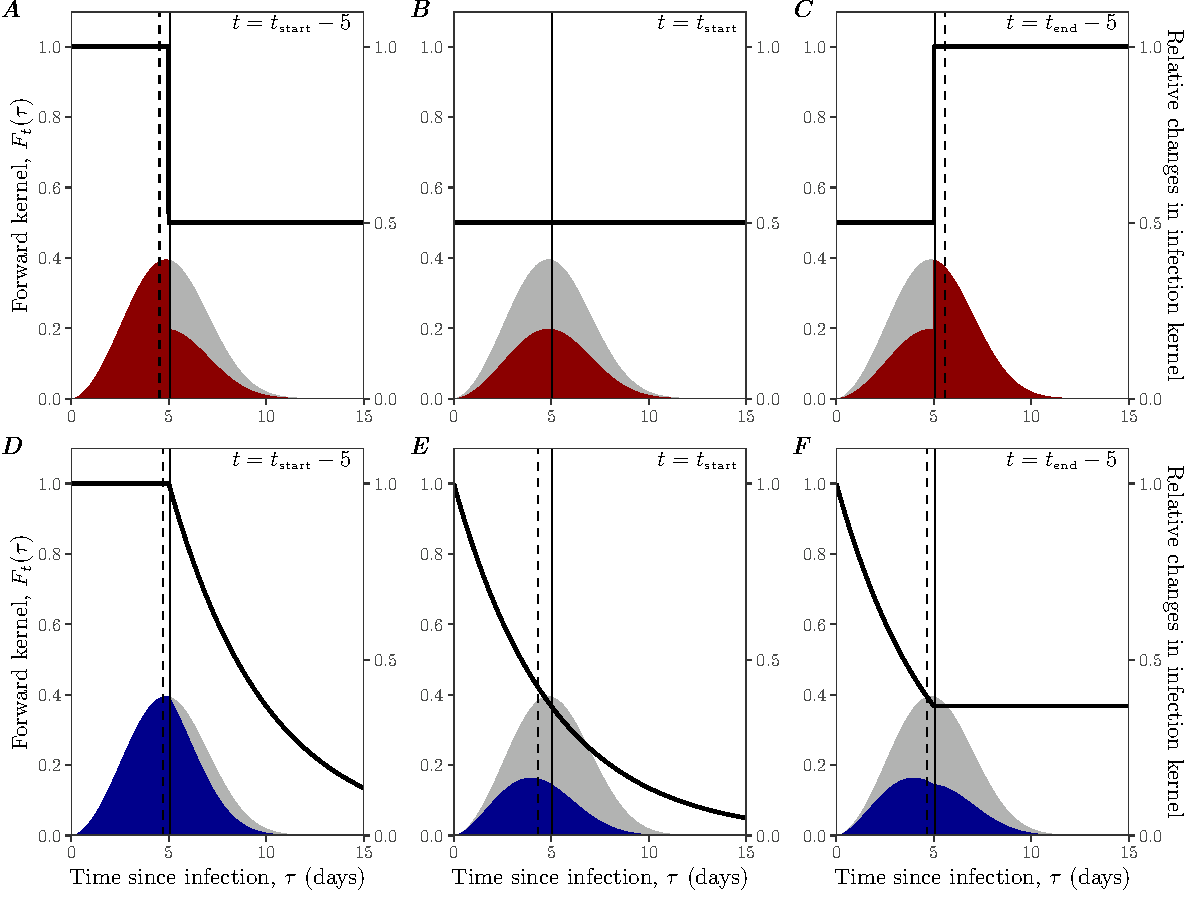
\includegraphics[width=1\textwidth]{pop_ind_compare.pdf}
\caption{
\textbf{The impact of constant-strength and constant-speed interventions on forward kernels.}
The impact of constant-strength (A--C) and constant-speed (D--F) intervention on forward kernels of cohort of individuals infected at different time:
5 days before intervention onset (A, D), during intervention (B, E), and 5 days before intervention offset (C, F).
Gray shaded curves represent the (fixed) intrinsic kernel $K_0(\tau)$, which is modeled using a gamma distribution with $\Ro$ of 2, a mean of 5 days and a squared coefficient of variation of 0.2.
Colored curves represent the forward kernel $F_t(\tau)$ under strength-based (A--C) and speed-based (D--F) interventions.
The strength-based intervention is assumed to reduce kernel by a factor of 2.
The speed-based intervention is assumed to have a constant hazard of $1/5/\textrm{days}$ during the intervention period.
Susceptible depletion is assumed to be negligible.
Solid black lines represent relative changes in the kernel: $F_t(\tau)/K_0(\tau)$.
Solid vertical lines show the (fixed) mean intrinsic generation interval and dashed vertical lines the mean forward generation interval.
}
\label{fig:indpop}
\end{figure}

To model changes in epidemic dynamics, we introduce an intervention function $\II(t, \tau)$ which can depend on both calendar time $t$ as well as time since infection $\tau$. 
Then, the infection kernel under $\II$ at calendar time $t$ can be written as:
\begin{equation}
K(t, \tau) = \Ro \II(t, \tau) g_0(\tau).
\end{equation}
Likewise, the forward kernel of an individual infected at time $t$ under $\II$ can be written as:
\begin{equation}
F_t(\tau) =  \Ro \II(t + \tau, \tau) g_0(\tau).
\end{equation}
The intervention function $\II(t, \tau)$ can capture any kinds of epidemiological changes, including changes in the susceptible pools $S(t)$ (either due to natural infection or vaccination) as well as introduction and lifting of non-pharmaceutical interventions.
Here, we focus on two idealized interventions, which we refer to as constant-strength and constant-speed interventions, and later generalize them to describe strength- and speed-like interventions \citep{dushoff2021speed}.
While our primary focuses are instantaneous quantities ($\Ri(t)$ and $g_t(\tau)$), we first illustrate the impact of constant-strength and constant-speed interventions using forward quantities as they describe realized transmission processes and are easier to interpret.

First, we consider a constant-strength intervention $\II(t, \tau) = \PP(t)$, which reduces the transmission rate by a constant amount across the age of infection $\tau$ at a given time $t$; note that $\PP(t)$ need not be constant across calendar time.
For example, a constant-strength intervention that reduces transmission by a factor of $\phi$ between time \tstart and \tend can be modeled as:
\begin{equation}
\PP(t) = \begin{cases}
1 & t < \tstart\\
\frac{1}{\phi} & \tstart \leq t < \tend\\
1 & \tend \leq t
\end{cases}.
\end{equation}
\fref{indpop}A--C illustrates the impact of such intervention on the forward kernel $F_t(\tau)$ of an individual infected 5 days before $\tstart$, at $\tstart$, and 5 days before $\tend$.
This constant-strength intervention reduces transmission immediately (\fref{indpop}A);
likewise, lifting this intervention can, in theory, can cause the forward kernel to return back to normal immediately (\fref{indpop}C).
Even though the exact shape of the kernel $F_t(\tau)$ depends on the time of infection and when the intervention was introduced relative to the infection time, the relative impact of intervention in reducing transmission (black solid lines in \fref{indpop}A--C, representing $F_t(\tau)/K(0, \tau)$) is constant ($1/\phi$) for transmission that occurs during the intervention period.

Such intervention has predictable effects on mean generation intervals:
implementing (lifting) intervention decreases (increases) future transmission potential and therefore decreases (increases) the mean forward generation interval (\fref{indpop}A,C).
If an individual is infected after \tstart (and much earlier than \tend), this intervention simply reduces the entire kernel by a constant amount and has no effect on realized generation intervals (\fref{indpop}B).
This observation generalizes the phenomenon of contraction of realized generation intervals due to susceptible depletion \citep{kenah2008generation,nishiura2010time,champredon2015intrinsic}.

Analogously, we consider a constant-speed intervention $\II(t, \tau) = \HH(t, \tau)$ that depends on time-varying hazard of isolation $h(t)$:
\begin{equation}
\HH(t, \tau) = \exp \left(- \int_0^\tau h(t-\sigma) \dsigma \right).
\end{equation}
Analogous to the constant-strength intervention, the constant-speed intervention assumes a constant hazard of isolation across the age of infection $\tau$ at a given time $t$; however, the hazard need not be constant across calendar time.
Then, $\HH(t,\tau)$ represents the probability that an individual infected $\tau$ time units ago has not been isolated by calendar time $t$.
In practice, the hazard of isolation is expected to depend not only on calendar time $t$ but also on the age of infection $\tau$---for example, we expect $h(t, \tau)$ to increase with $\tau$ for symptom-based interventions to reflect the increasing cumulative probability of developing symptoms.

For example, a constant-speed intervention that takes place between time \tstart and \tend can be modeled using the following hazard function:
\begin{equation}
h(t) = \begin{cases}
0 & t < \tstart\\
\theta & \tstart \leq t < \tend\\
0 & \tend \leq t
\end{cases}.
\end{equation}
In this case, the probability that an individual infected at time $t$ has not been isolated by $\tau$ time units after infection depends on the amount of time the individual has been exposed to this intervention.
If the individual is infected before $\tstart$, they will not be isolated by this intervention until after $\tstart$.
If the individual is infected after $\tend$, they will never be isolated by this intervention.
\fref{indpop}D--E illustrates the impact of such intervention on the forward kernel of an individual infected 5 days before $\tstart$, at $\tstart$, and 5 days before $\tend$.
Unlike the constant-strength intervention, the constant-speed intervention does not show effects immediately;
that is, the rate at which an infected individual generates secondary infections at time $\tstart$ remains unaffected by the intervention because it takes time to identify and isolate infected individuals.
On the other hand, when the intervention is lifted at $\tend$, the value of the kernel at calendar time remains unchanged because some fraction of infected individuals have already been isolated.
The constant-speed interventions always shorten realized generation intervals because they prevent late transmission (\fref{indpop}D--E).

Finally, we can decompose the generalized intervention function $\II(t, \tau)$ as a product of constant-strength and constant-speed interventions: $\II(t, \tau) = \PP(t) \HH(t, \tau)$. 
Then, the dynamics of incidence $i(t)$ can be written as:
\begin{align}
i(t) &= \Ro \PP(t) \int_0^\infty \HH(t, \sigma) g_0(\sigma) i(t-\sigma)\dsigma.
\end{align}
In this case, the instantaneous reproduction number and generation-interval distributions are given by:
\begin{align}
\Ri(t) &= \RR_0 \PP(t) \int_0^\infty \HH(t,\sigma) g_0(\sigma) \dsigma,\\
g_t(\tau) &= \frac{\HH(t,\tau) g_0(\tau)}{\int_0^\infty \HH(t,\sigma) g_0(\sigma) \dsigma},
\end{align}
which allow us to express the renewal equation in the form of \eref{renewal_instantaneous}.
Therefore, the instantaneous generation-interval distribution changes under constant-speed interventions but not under constant-strength interventions, even though both types of interventions affect the realized generation-interval distribution.

\subsection{Quantifying changes in generation-interval distributions}
\label{ss:instg}

In order to model the renewal process, we have to know how the instantaneous generation-interval distribution $g_t(\tau)$ changes across time $t$.
The instantaneous distribution measures the infectiousness of an individual infected $\tau$ time units ago at time $t$ and is therefore different from the distribution of realized generation intervals (i.e., time between actual infection events).
For example, while both the forward generation-interval distribution $f_{t-\tau}(\tau)$ and the instantaneous generation-interval distribution $g_t(\tau)$ depend on the rate at which secondary cases at time $t$ are generated by a primary case infected at time $t-\tau$, $K(t, \tau)$, they are normalized by different quantities:
\begin{equation}
f_{t-\tau}(\tau) = \frac{K(t,\tau)}{\int_0^\infty K(t-\tau+\sigma,\sigma) \dsigma} \neq \frac{K(t,\tau)}{\int_0^\infty K(t,\sigma) \dsigma} = g_t(\tau).
\end{equation}
The forward distribution $f_{t-\tau}(\tau)$ is normalized by the average number of new infections caused by an individual infected at time $t-\tau$ (i.e., the case reproduction number, $\Rc(t-\tau)$).
On the other hand, the instantaneous distribution $g_t(\tau)$ is normalized by a counterfactual measure of transmission $\Ri(t)$.

Rewriting \eref{fkernel} provides further insight into their differences:
\begin{equation}
f_t(\tau) = \frac{\Ri(t + \tau) g_t(\tau, \tau)}{\int \Ri(t + \sigma) g_{t+\sigma}(\sigma) \dsigma}.
\end{equation}
Even if the instantaneous generation-interval distribution $g_t(\tau)$ remains invariant across time (i.e., $g_t(\tau) = g_0(\tau)$), changes in transmission conditions (therefore, $\Ri(t)$) are expected to change the shape of the forward generation-interval distribution;
for example, as we showed earlier, the instantaneous generation-interval distribution does not change under the constant-strength intervention, but the forward generation-interval distribution changes.
Therefore, renewal equation models that rely on the forward form (\eref{renewal_forward}) but assume time-invariant $f_t(\tau)$ should generally be avoided.

On the other hand, if we were to take all realized generation intervals that end at time $t$ and form a distribution, we obtain what is known as the backward generation-interval distribution, $b_t(\tau)$:
\begin{equation}
b_t(\tau) = \frac{i_{t-\tau}(t)}{\int_0^\infty i_{t-\sigma}(t) \dsigma}.
\label{eq:backward}
\end{equation}
The backward distribution systematically differs from the instantaneous distribution:
\begin{equation}
b_t(\tau) = \frac{g_t(\tau) i(t-\tau)}{\int_0^\infty g_t(\sigma) i(t-\sigma) \dsigma}
\label{eq:b1}
\end{equation}
due to its dependence on previous incidence of infection.
For example, when incidence is increasing exponentially, we are more likely to observe shorter generation intervals for a cohort of infectees that were infected at the same time because their infectors are more likely to have been infected recently.

Rewriting \eref{b1} in terms of the forward distribution shows that the backward distribution also depends on the case reproduction number $\Rc(t-\tau)$ of the cohort of infectors at time $t-\tau$:
\begin{equation}
b_t(\tau) = \frac{\Rc(t-\tau) f_{t-\tau}(\tau) i(t-\tau)}{\int_0^\infty \Rc(t-\sigma) f_{t-\sigma}(\sigma) i(t-\sigma) \dsigma}.
\label{eq:b2}
\end{equation}
As defined in \eref{backward}, the total density of generation intervals between time $t-\tau$ and time $t$ corresponds to $i_{t-\tau}(t)$ (i.e., the total number of infections at time $t$ caused by a cohort of individuals that were infected at time $t-\tau$), which depends on the incidence $i(t-\tau)$ at time $t-\tau$ as well as their average infectiousness $\Rc(t-\tau)$.
In other words, a cohort of infectors that generated more infections will have greater contribution towards the backward generation-interval distribution at a given time.
Several studies have noted, in various contexts, that backward distributions of epidemiological delays provide biased estimates of the forward distribution due to effects of this sort \citep{nishiura2010time,champredon2015intrinsic,park2020inferring,park2020forward}.

\subsection{Quantifying changes in reproduction numbers}

The instantaneous reproduction number $\Ri(t)$ provides a measure for the impact of intervention:
\begin{align}
\Ri(t) &= \int_0^\infty K(t, \sigma) \dsigma, \\
&= \RR_0 S(t) \PP(t) \int_0^\infty \HH(t,\sigma) g_0(\sigma) \dsigma.
\label{eq:rt}
\end{align}
Since $\Ri(t)$ measures conditions at time $t$, one would typically expect to detect changes in $\Ri(t)$ as soon as interventions are implemented---as we see in \eref{rt} (and also in \fref{indpop}), this is true for changes in a constant-strength intervention $\PP(t)$ but not under a constant-speed intervention $\HH(t, \sigma)$.
Therefore, it has been previously argued that $\Ri(t)$ can provide a real-time measure for whether the disease will continue to spread or not \citep{gostic2020practical}.

Estimating $\Ri(t)$ depends on the instantaneous generation-interval distribution $g_t(\tau)$,
which can vary across time under constant-speed interventions:
\begin{equation}
g_t(\tau) = \frac{K(t, \tau)}{\RR(t)} = \frac{\HH(t,\tau) g_0(\tau)}{\int_0^\infty \HH(t,\sigma) g_0(\sigma) \dsigma}.
\end{equation}
By rearranging \eref{renewal}, we obtain the following estimator for $\RR(t)$:
\begin{equation}
\Ri(t) = \frac{i(t)}{\int_0^\infty g_t(\sigma) i(t-\sigma) \dsigma}.
\end{equation}
While this estimator is similar in form to previously proposed estimators \citep{fraser2007estimating}, it differs in allowing for the underlying instantaneous generation-interval distribution to vary across time.
In particular, the popular R package \texttt{EpiEstim}, \cite{cori2013new} uses the approach while assuming that the underlying instantaneous distribution does not change over time; 
such methods accurately estimate changes in $\Ri(t)$ under constant-strength interventions, but not necessarily under more general conditions.

When both strength- and speed-like interventions are present during an ongoing epidemic, classical estimators \cite{fraser2007estimating,cori2013new} measure a slightly different quantity:
\begin{equation}
\Rcori(t) = \frac{i(t)}{\int_0^\infty g_0(\sigma) i(t-\sigma) \dsigma}.
\end{equation}
This is the number of infections per infection required to explain current incidence under the counter-factual that the generation-interval distribution has not changed.
This estimator is widely used, because it is simple, often robust to estimate, and often a good proxy for \Ri.
When interventions have speed-like components, however, the exact meaning of this estimator can be difficult to interpret; 
and it does not necessarily accurately reflect how conditions are changing through time.
\swp{I feel that we're better off deleting these now: \old{In addition, $\Rcori(t)=1$ does not necessarily serve as a threshold value.
When conditions remain roughly constant over a long term, both $\Ri(t) = 1$ and $\Rcori(t)=1$ serve as a threshold condition since $\Ri(t) = 1$ holds for $r=0$ regardless of the underlying generation-interval distribution. 
However, when conditions are changing rapidly, $\Rcori(t)=1$ does not necessarily provide a threshold condition---we revisit this point later in text.}}

The case reproduction number $\Rc(t)$ is similarly complicated. 
Since $\Rc(t)$ measures the average number of new infections caused by an individual infected at time $t$, we have
\begin{equation}
\Rc(t) = \frac{\int_0^\infty i_t(t+\sigma) \dsigma}{i(t)},
\end{equation}
where $i_t(t+\sigma)$ represents incidence at time $t+\sigma$ caused by individuals who were infected at time $t$.
Substituting \eref{backward}, it is straightforward to see that $\Rc(t)$ can be estimated by using the backward generation-interval distribution:
\begin{equation}
\Rc(t) = \frac{\int_0^\infty b_{t+\sigma}(\sigma) i(t+\sigma) \dsigma}{i(t)}.
\end{equation}
Here, the numerator, which represents the total number of infections caused by individuals infected at time $t$, is calculated by multiplying future incidence $i(t+\sigma)$ with the probability that future infections are caused by an individual infected at time $t$ $b_{t+\sigma}(\sigma)$.
Using \eref{b1}, we obtain a Wallinga-Teunis-like estimator \citep{wallinga2004different}:
\begin{equation}
\Rc(t) = \int_0^\infty \left(\frac{g_{t+\sigma}(\sigma) i(t+\sigma)}{\int_0^\infty g_{t+\sigma}(\sigma') i(t+\sigma-\sigma') \dsigma'} \right) \dsigma.
\label{eq:wtlike}
\end{equation}
This derivation clarifies that, like the classic estimator for \Ri, the classic estimator for \Rc\ is based on the instantaneous generation-interval distribution, and thus implicitly relies on the assumption that changes in transmission are strength-like and not speed-like.

% This derivation also shows that, when the instantaneous generation-interval distribution is unknown, $\Rc(t)$ can be estimated from backward generation-interval distributions, which, in some cases can be estimated from contact tracing.
% If realized serial intervals (i.e., time between symptom onset of the infector and the infectee) are observed instead, a similar calculation can be done using the estimated backward serial-interval distribution, to estimate a case-reproduction number for a different cohort: a cohort of individuals who developed symptoms at a given time. This is the serial reproduction number \cite{park2020forward}.
% In contrast, the Wallinga-Teunis-like estimator \eref{wtlike} cannot be used for serial intervals because the corresponding time-independent instantaneous distributions cannot be properly defined \jd{I think this is what you are trying to say. Is it possible to explain concisely why they can't be defined?}

Some studies have suggested substituting the forward distribution $f_t(\tau)$, including the forward serial-interval distribution, instead to estimate the ``time-varying'' or the ``effective'' reproduction number $\RR(t)$ \citep{liu2018measurability, ali2020serial}:
\begin{equation}
\tsub{\RR}{forward}(t) = \frac{i(t)}{\int_0^\infty i(t-\sigma) f_{t-\sigma}(\sigma) \dsigma}.
\end{equation}
This choice is potentially problematic, as the forward distribution differs systematically from the instantaneous distribution.
For example, under constant-strength interventions, the forward distribution changes over time even though the instantaneous distribution remains time invaraint---these differences can lead to systematic biases.
In Section 3, we compare $\tsub{\RR}{forward}(t)$ with $\Ri(t)$ and $\Rc(t)$.

\subsection{Quantifying changes in time-dependent growth rate}

The instantaneous reproduction number $\Ri(t)$ provides a long-term threshold for whether the epidemic will \emph{eventually} grow or decline if current conditions remain unchanged;
perhaps counterintuitively, it does not tell us whether the epidemic is growing or not at a given moment.
Instead, if we want to quantify whether incidence is increasing or decreasing, we can simply calculate the epidemic growth rate.
Researchers often focus on the initial exponential growth rate, but we can look at the per-capita growth rate at any time:
\begin{equation}
r(t) = \frac{1}{i(t)} \frac{\dd{i(t)}}{\dd{t}}.
\end{equation}
By definition, incidence grows when $r(t) > 0$ (and vice versa)---thus, this provides an instantaneous threshold for incidence of infection (but does not provide information about the long-term behavior).

\section{Example: Semi-mechanistic SIR model}

In order to understand how constant-strength and constant-speed interventions affect disease spread, we use a semi-mechanistic SIR model to generate synthetic data and compare various estimates of $\RR(t)$ and $r(t)$:
\begin{align}
\frac{\dd{S}}{\dd{t}} &= - \beta(t)S I, \label{eq:dSdt}\\
\frac{\dd{I}}{\dd{t}} &= \beta(t)S I - \gamma(t) I,\\
\frac{\dd{R}}{\dd{t}} &= \gamma(t) I,  \label{eq:dRdt}
\end{align}
where $S$, $I$, $R$ represent proportion of individuals that are susceptible, infected, and removed (either due to recovery or isolation measures);
$\beta(t)$ represent time-varying transmission rate; and $\gamma(t)$ represent time-varying removal rate.
We refer to this model as semi-mechanistic because the infection and recovery process are modeled explicitly, but changes in $\beta$ and $\gamma$ are allowed to change freely over time (without any mechanisms).
In this case, the instantaneous kernel can be written as:
\begin{equation}
K(t, \tau) = \beta(t) S(t) \exp\left(-\int_{t-\tau}^t \gamma(s) \dd{s} \right).
\end{equation}
We see that changes in transmission rate $\beta(t)$ and removal rate $\gamma(t)$ exactly match the definitions of constant-strength and constant-speed interventions.
In particular, abrupt changes in $\gamma(t)$ will not affect the incidence immediately due to delays in isolating individuals.
Finally, the instantaneous reproduction number is given by:
\begin{equation}
\Ri(t) = \beta(t) S(t) \int_0^\infty \exp\left(-\int_{t-\tau}^t \gamma(s) \dd{s} \right) \dtau.
\end{equation}
When $\gamma(t) = \gamma(0)$, we obtain a familiar form: $\Ri(t) = \Ro S(t)$,
where $\Ro = \beta(0)/\gamma(0)$.

\begin{figure}[!ht]
\includegraphics[width=\textwidth]{figure_beta_gamma.pdf}
\caption{
\textbf{Assumed changes in transmission and removal rate.}
The semi-mechanistic SIR model is simulated under two different scenarios.
(A) Equivalent strength-based intervention scenario.
Removal rate $\gamma$ is fixed to $0.2\pday$ throughout.
(B) Equivalent speed-based intervention scenario.
Transmission rate $\beta$ is fixed to $0.3\pday$ throughout.
(C) Instantaneous incidence under equivalent strength- and speed-based intervention scenarios.
(D) Growth rate estimates over time.
Equivalent strength- and speed-based scenarios give identical incidence trajectories.
}
\label{fig:assumption}
\end{figure}

Here, we compare two different scenarios, in which interventions are introduced and are later partially lifted (\fref{assumption}).
First, we consider a smooth introduction and lifting of a constant-strength intervention, modeled by changes in $\beta$ while fixing $\gamma$ (\fref{assumption}A).
Next, we consider a sudden introduction and lifting of a constant-speed intervention, modeled by changes in $\gamma$ while fixing $\beta$ (\fref{assumption}B).
We refer to these two interventions as \emph{equivalent} constant-strength and constant-speed interventions because they give identical incidence curves (\fref{assumption}C), demonstrating that changes in $\beta$ and $\gamma$ cannot be jointly identified from the incidence curve alone (see Methods and Materials).
In both cases, growth rate $r(t)$ estimates are identical (\fref{assumption}D); as we show later, however, changes in reproduction numbers differ between the two scenarios.

\begin{figure}[!th]
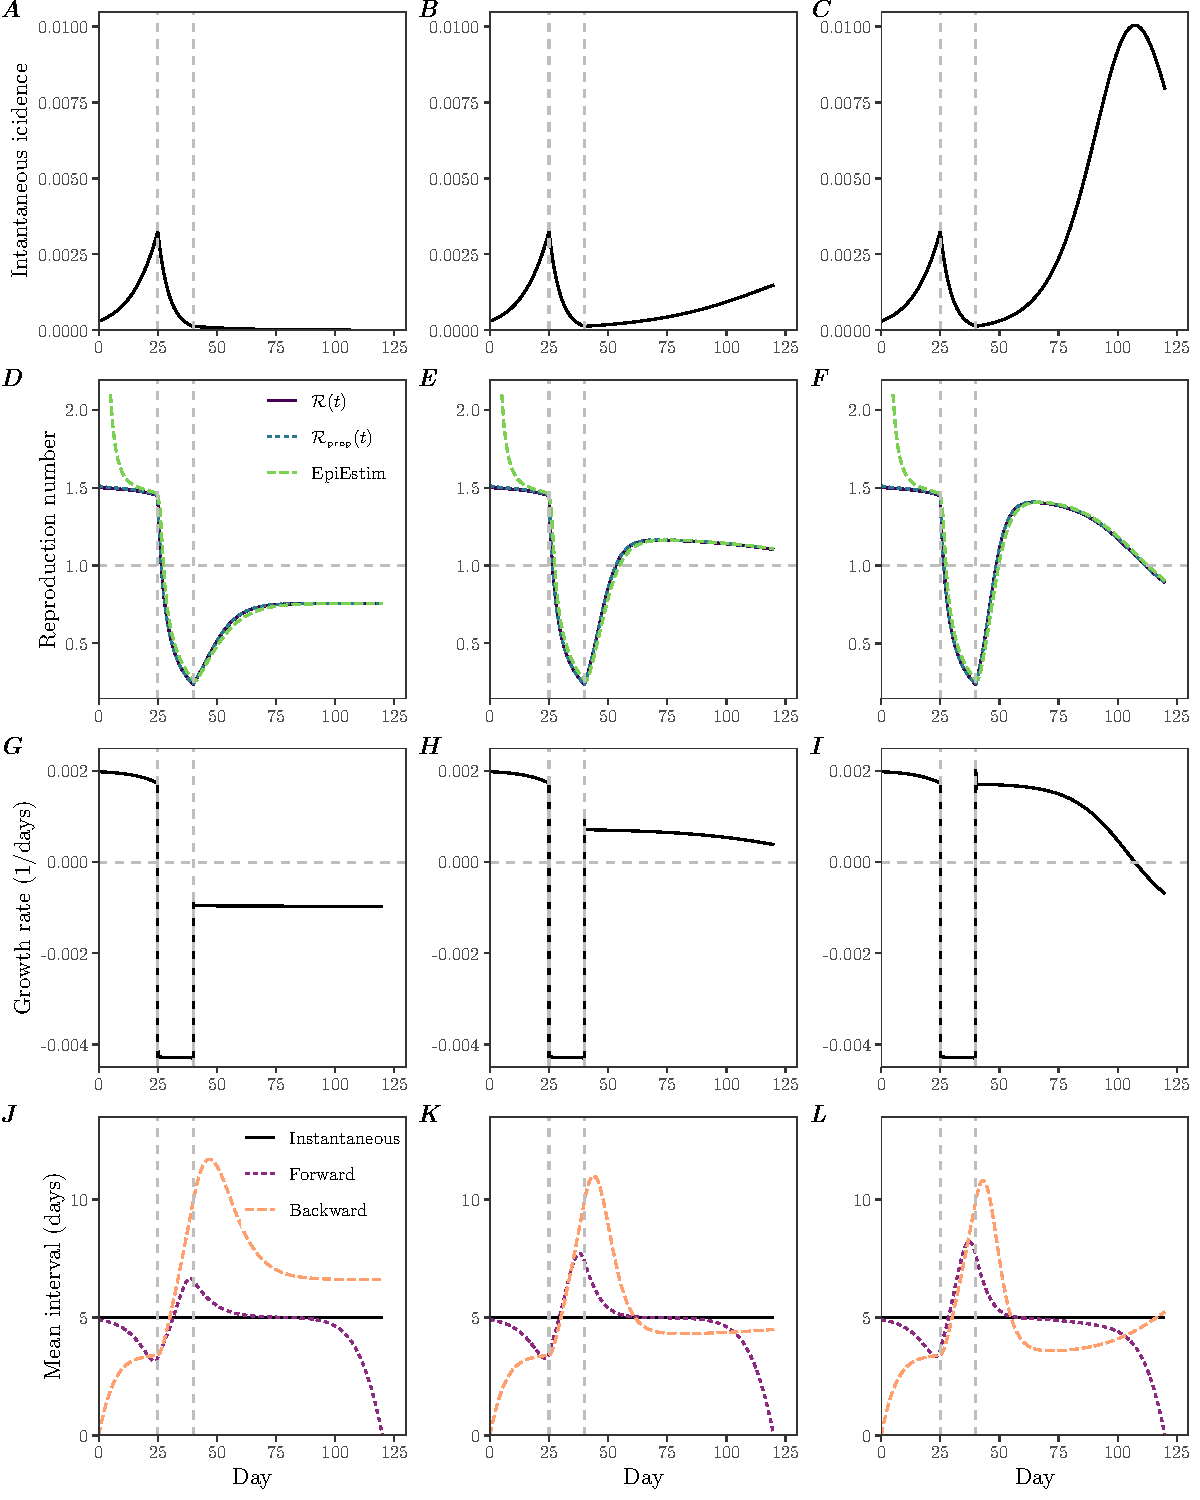
\includegraphics[width=\textwidth]{figure_sir_beta.pdf}
\caption{
\textbf{Epidemiological dynamics of a semi-mechanistic SIR model under equivalent strength-based intervention.}
(A) Changes in true instantaneous reproduction number $\Ri(t)$, proportional reproduction number $\Rcori(t)$, estimated $\Ri(t)$ using EpiEstim (assuming a population of one million), and estimated $\tsub{\RR}{forward}(t)$ using the forward generation-interval distribution.
(B) Changes in true case reproduction number $\Rc(t)$, estimated $\Rc(t)$ using Wallinga-Teunis estimator with intrinsic generation-interval distribution, and estimated $\tsub{\RR}{forward}(t)$ using the forward generation-interval distribution.
(C) Changes in mean instantaneous, forward, and backward generation intervals.
}
\label{fig:sir_beta}
\end{figure}

Epidemiological dynamics under a constant-strength intervention are presented in \fref{sir_beta}.
In this case, the proportional reproduction number $\Rcori(t)$, which relies on the intrinsic generation-interval distribution, matches the instantaneous reproduction number $\Ri(t)$, which relies on the instantaneous generation-interval distribution (\fref{sir_beta}A).
Therefore, we are able to correctly estimate $\Ri(t)$ using \texttt{EpiEstim} (\fref{sir_beta}A).
The initial overestimation from \texttt{EpiEstim} is caused by the left censoring \citep{gostic2020practical}.
Minor differences between \texttt{EpiEstim} estimates and $\Rcori(t)$ are caused by discretization.

Likewise, we can accurately estimate the case reproduction number $\Rc(t)$ using the classic Wallinga-Teunis estimator (based on the intrinsic generation-interval distribution) (\fref{sir_beta}B).
This is because the instantaneous generation-interval distribution does not change over time under constant-strength interventions (\fref{sir_beta}C).
Using the forward generation-interval distribution, instead of the instantaneous generation-interval distribution, matches neither $\Ri(t)$ ($\tsub{\RR}{forward}(t)$ in \fref{sir_beta}A) nor $\Rc(t)$ in this case ($\tsub{\RR}{forward}(t)$ in \fref{sir_beta}B) because the forward distribution changes, even when the instantaneous distribution does not change (\fref{sir_beta}C).
As described earlier (\fref{indpop}A--C), introducing and lifting a constant-strength intervention cause the forward generation intervals become shorter and longer, respectively (\fref{sir_beta}C);
the backward distribution exaggerates these changes \jd{This confuses me. Is it clear in what sense backward depends on forward (rather than on shared drivers)?} it depends on the forward distributions as well as previous incidence.
The mean backward generation interval begins from 0 days in this case due to left censoring.

\begin{figure}
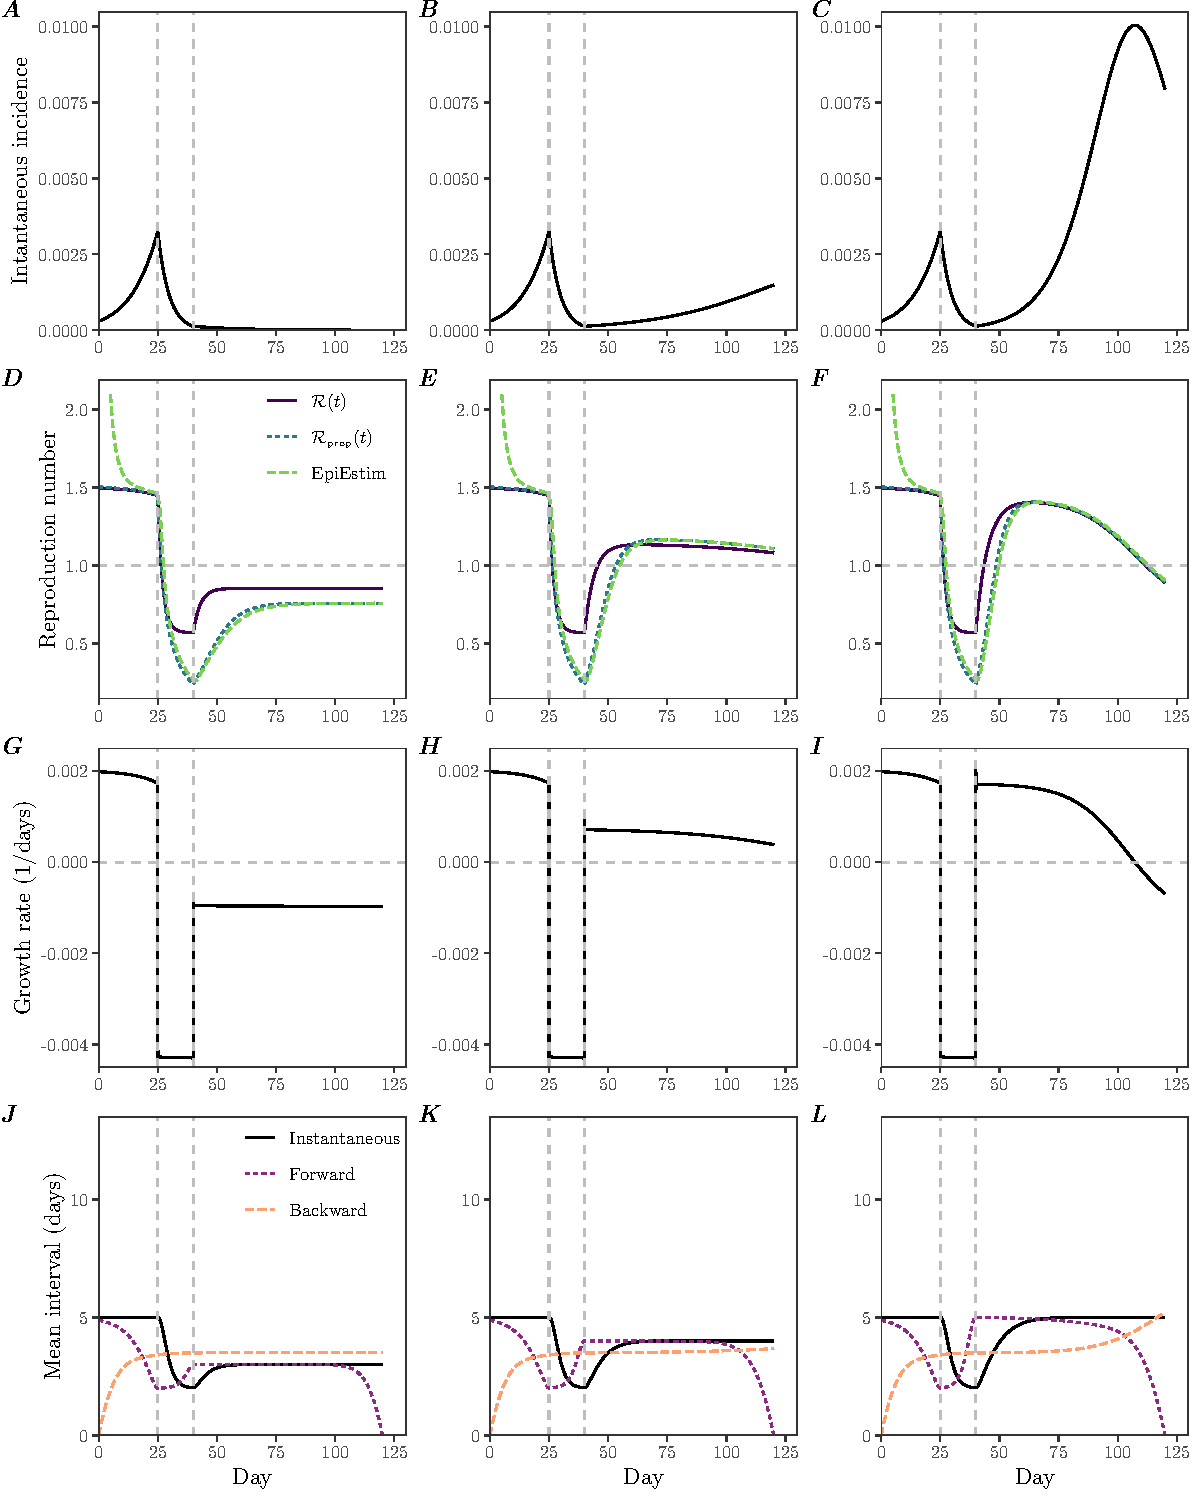
\includegraphics[width=\textwidth]{figure_sir_semi.pdf}
\caption{
\textbf{Epidemiological dynamics of a semi-mechanistic SIR model under equivalent speed-based intervention.}
(A) Changes in true instantaneous reproduction number $\Ri(t)$, proportional reproduction number $\Rcori(t)$, estimated $\Ri(t)$ using EpiEstim (assuming a population of one million), and estimated $\tsub{\RR}{forward}(t)$ using the forward generation-interval distribution.
(B) Changes in true case reproduction number $\Rc(t)$, estimated $\Rc(t)$ using Wallinga-Teunis estimator with intrinsic generation-interval distribution, and estimated $\tsub{\RR}{forward}(t)$ using the forward generation-interval distribution.
(C) Changes in mean instantaneous, forward, and backward generation intervals.
}
\label{fig:sir_semi}
\end{figure}

Epidemiological dynamics under a constant-speed intervention are presented in \fref{sir_semi}.
In this case, the instantaneous generation-interval distribution changes through time.  
$\Rcori(t)$ differs from the true $\Ri(t)$ (\fref{sir_semi}A) because the constant-speed interventions lead to changes in the instantaneous generation-interval distribution (\fref{sir_semi}C).
Therefore, \texttt{EpiEstim} inaccurately estimates $\Ri(t)$ (\fref{sir_semi}A)---
in particular, \texttt{EpiEstim} estimates that $\Ri(t)$ crossed the threshold $\Ri(t)=1$ later (around $t=55$) than it actually did (around $t=45$).

Using the intrinsic distribution is also problematic for estimating the case reproduction number $\Rc(t)$ (\fref{sir_semi}B).
The true $\Rc(t)$ changes sharply, reflecting sharp changes in the removal rate $\gamma(t)$ (\fref{assumption}B), but using the intrinsic distribution gives smooth estimates of $\Rc(t)$.
In this case, $\tsub{\RR}{forward}(t)$ matches $\Ri(t)$ and $\Rc(t)$ better than their corresponding estimates using the intrinsic generation-interval distribution (EpiEstim and Wallinga-Teunis in \fref{sir_semi}, respectively) because the forward generation-interval distribution captures the effects of the constant-speed intervention (\fref{sir_semi}C).
Surprisingly, the backward generation-interval distribution stays nearly constant because the effect of decreasing incidence (which lengthens the backward generation intervals) cancels out with that of shorter realized generation intervals, caused by the constant-speed intervention (\fref{sir_semi}C).

Comparing simulations under equivalent constant-strength and constant-speed interventions allows us to better understand the differences between the $\Ri(t)$ and $r(t)$ in capturing current conditions at time $t$.
Under a constant-strength intervention, $\Ri(t) = \beta(t)/\gamma(0)$, and therfore $\Ri(t)$ crosses the threshold, $\Ri(t) = 1$, when $\beta(t)$ crosses the threshold, $\beta(t) = \gamma(0)$ (compare \fref{assumption}A with \fref{sir_beta}A).
Under a constant-speed intervention, however, sharp changes in $\gamma(t)$ translate to smooth changes in $\Ri(t)$, and therefore $\Ri(t)$ crosses the threshold, $\Ri(t) = 1$, later (compare \fref{assumption}B with \fref{sir_semi}A).
Instead, sharp changes in $\gamma(t)$ are captured by sharp changes in $r(t)$ (compare \fref{assumption}B with \fref{assumption}D)---this can readily seen by deriving an explicit expression for $r(t)$:
\begin{align}
r(t) &=  \frac{1}{i(t)} \frac{\dd i(t)}{\dd t}\\
&= \frac{1}{\beta(t)} \frac{\dd \beta(t)}{\dd t} - \beta(t) I + \beta(t) S - \gamma(t) \label{eq:explicitrt}
\end{align}
where the instantaneous incidence corresponds to $i(t) = \beta(t) S I$ for the semi-mechanistic SIR model.
\eref{explicitrt} also shows that changes in $\beta(t)$ is going to have non-trivial effects on $r(t)$, which depend not only on $\beta(t)$ itself but also on per-capita changes in $\beta(t)$ and both state variables, $S$ and $I$.
Therefore, $\Ri(t)$ is the best measure for capturing current conditions at time $t$ under constant-strength interventions, whereas $r(t)$ is the best measure for capturing current conditions at time $t$ under constant-speed interventions. 

\section{Discussion}

The impact of epidemic interventions are often characterized by changes in ``effective'' reproduction numbers, $\RR(t)$.
Despite historical emphasis on estimating $\RR(t)$, current frameworks neglect possibility that the underlying generation-interval distribution can change over time---an insight that goes back $>10$ years \citep{fraser2007estimating}.
Here, we distinguish two reproduction numbers---instantaneous reproduction number $\Ri(t)$ and case reproduction number $\Rc(t)$, which describe counterfactual and realized transmission processes, respectively---and show that both reproduction numbers can correctly describe the renewal process of infection when paired with correct generation-interval distributions.
In particular, a counterfactual generation-interval distribution, which we refer to as the instantaneous generation-interval distribution, is required to correctly estimate the instantaneous reproduction number. 
This distribution is affected by constant-speed, but not constant-strength, interventions.
Neglecting changes in this distribution gives biased estimates of $\Ri(t)$, including estimates of when $\Ri(t)$ crosses the threshold value of 1.
Instead, time-dependent growth rate $r(t)$ is a better measure for characterizing the impact of epidemic intervention under a constant-speed intervention.

In practice, estimating the instantaneous generation-interval distribution is expected to be difficult as it systematically differs from the realized generation intervals: even if we can observe all realized generation intervals throughout an epidemic, estimating the instantaneous distribution $g(t, \tau)$ is not trivial.
For example, even within a homogeneously mixing population, in which the disease is allowed to spread unchecked (and therefore $g(t, \tau) = g_0(\tau)$ for all $t$), aggregating all realized generation intervals underestimates the mean intrinsic generation interval due to susceptible depletion \citep{park2020inferring}.
Novel statistical methods are needed to accurately estimate the instantaneous distribution $g(t, \tau)$.

Most state-of-art statistical softwares for estimating reproduction numbers assume that the instantaneous generation-interval distribution does not change across time (e.g., \citep{10.12688/wellcomeopenres.16006.2,flaxman2020estimating,brauner2021inferring}).
We refer to these estimates as proportional reproduction number $\Rcori$ as they capture proportional reduction in incidence, rather than transmission.
While this may be the most parsimonious and best available approach for estimating $\mathcal R(t)$, we encourage researchers to not overemphasize the value of this reproduction number estimate, especially whether it crosses the threshold value or not---in particular, this reproduction number estimate can differ systematically from the true instantaneous reproduction number $\Ri$ under speed-like interventions such as contact tracing.
Emergence of new variants with a different infectiousness profile (and therefore the intrinsic generation-interval distribution) is expected to have similar effects.

In the context of the current SARS-CoV-2 pandemic, assuming a time-invariant generation-interval distribution could have been justified during the early period given that most interventions were strength-like, including lockdowns, school closures, and travel bans \citep{flaxman2020estimating,li2021temporal,brauner2021inferring}.
Nonetheless, speed-like  interventions, including intense contact tracing efforts \citep{park2020contact} and introduction of contact tracing apps \citep{wymant2021introduction}, had clear, non-negligible impact on the overall spread;
these interventions, including awareness-driven behavioral changes (which can cause symptomatic individuals to self-isolate faster), are likely to have shortened the instantaneous generation intervals by preventing transmission during later stages of infection.
Therefore, current estimates of $\Ri$ which relies on early estimates of the generation-interval distributions may be biased and reassessed.
Future studies should also consider incorporating hazard-based changes for modeling speed-like interventions.

Our study highlights the value of growth rates $r(t)$ in characterizing epidemic spread \citep{abbott2020temporal,anderson2020reproduction}.
\swp{need to rewrite this paragraph}
% The instantaneous reproduction number $\Ri(t)$ tell us whether the epidemic will continue to grow if conditions remain the same but does not tell us whether the epidemic is growing or not at a given moment.
% In contrast, $r(t)$ provides a robust measure of whether incidence is growing or decreasing at a given time under both strength- and speed-based interventions;
% but it does not provide information about future epidemic dynamics.
% \cite{parag2021epidemic} recently argued that $\RR(t)=1$ correspond to $r(t) = 0$ under correct assumptions about pathogen transmission and that $\RR(t)$ is theoretically more informative---however, we argue that this conclusion depends on their assumption to link $\RR(t)$ and $r(t)$ via the generation-interval distribution, an assumption that holds only when conditions remain constant.
% As we show here, this is not the case when conditions are changing---that is, the sign of $r(t)$ does not need to correspond to whether $\RR(t)$ is greater or less than 1.
% Time-varying reproduction number $\RR(t)$ and growth rate $r(t)$ encompass different information and should be used as complementary measures for describing epidemic dynamics \citep{dushoff2021speed}.

The renewal equation framework based on the instantaneous form (\eref{renewal_instantaneous}) has been widely used in epidemic modeling due to its flexibility.
A few studies relied on the forward form (\eref{renewal_forward}), but they incorrectly assumed a time-invariant generation-interval distribution \citep{nishiura2007time,alvarez2020variational,white2021statistical}.
As we show here, the forward generation-interval distributions, which change over time as transmission conditions change, correctly links the renewal process when paired with the case reproduction number.
To our knowledge, this is the first study to correctly link the case reproduction number with the forward renewal equation and to demonstrate the equivalence between the forward and instantaneous renewal formulations---
even when the case reproduction number was first introduced by \cite{wallinga2004different}, they did not explicitly link the case reproduction number to the renewal process.
Our study provides theoretical foundation for modeling epidemic processes.

\swp{Jonathan, can you try writing the last paragraph of the discussion?}

\section{Methods}

\subsection{Equivalent strength- and speed-based interventions}

Here, we model a simple scenario in which a flu-like pathogen with $\Ro = 1.5$ invades an immunologically naive population using the semi-mechanistic SIR model (\eref{dSdt}--\eref{dRdt}).
We begin by modeling speed-based intervention and find the equivalent strength-based intervention.  
In particular, we assume that the disease spreads without any intervention in the beginning;
on day 25, an intense case isolation measure is implemented; and
on day 40, the intervention is partially lifted.
This is modeled as follows:
\begin{equation}
\beta(t) = 3/10\,\,\textrm{days}^{-1}, \gamma(t) = \begin{cases}
1/5\,\, \textrm{days}^{-1} & t < 25\\
1/2\,\, \textrm{days}^{-1} & 25 \leq t < 40 \\
1/4\,\, \textrm{days}^{-1} & 40 \leq t
\end{cases}.
\end{equation}
Simulations are run for 100 days based on the following initial conditions: $S(0) = 1 - 10^{-3}$, $I(0) = 10^{-3}$, and $R(0) = 0$.

Since we assume that incidence is known exactly until time $t^\ast$, we can, in fact, estimate the transmission rate $\beta^\ast(t)$ (with fixed $\gamma(t)=\gamma(0)$) that gives identical incidence trajectory until time $t^\ast$.
This transmission rate is given by:
\begin{equation}
\beta^\ast(t) = \frac{\Rcori(t)\gamma(0)}{S(t)},
\end{equation}
where the proportional reproduction number $\Rcori$ is calculated from the incidence curve $i(t)$.
More generally, given true incidence $i(t)$ until time $t^\ast$, modulated by any combination of strength- and speed-based interventions, we can find equivalent strength-based intervention $\PP^\ast(t)$ until time $t^\ast$:
\begin{equation}
\PP^\ast(t) = \frac{\Rcori(t)}{\Ro S(t)},
\end{equation}
which generates an identical incidence curve when the initial conditions are identical.

\bibliography{individual_intervention}

\end{document}
